\section{SimSite3D::geometry::two\_\-thirds\_\-triangle Class Reference}
\label{classSimSite3D_1_1geometry_1_1two__thirds__triangle}\index{SimSite3D::geometry::two_thirds_triangle@{SimSite3D::geometry::two\_\-thirds\_\-triangle}}
Simple derived class that gives us a unique number for 2/3rds of triangle.  


{\tt \#include $<$Immovable\-Trimesh.H$>$}

Inheritance diagram for SimSite3D::geometry::two\_\-thirds\_\-triangle::\begin{figure}[H]
\begin{center}
\leavevmode
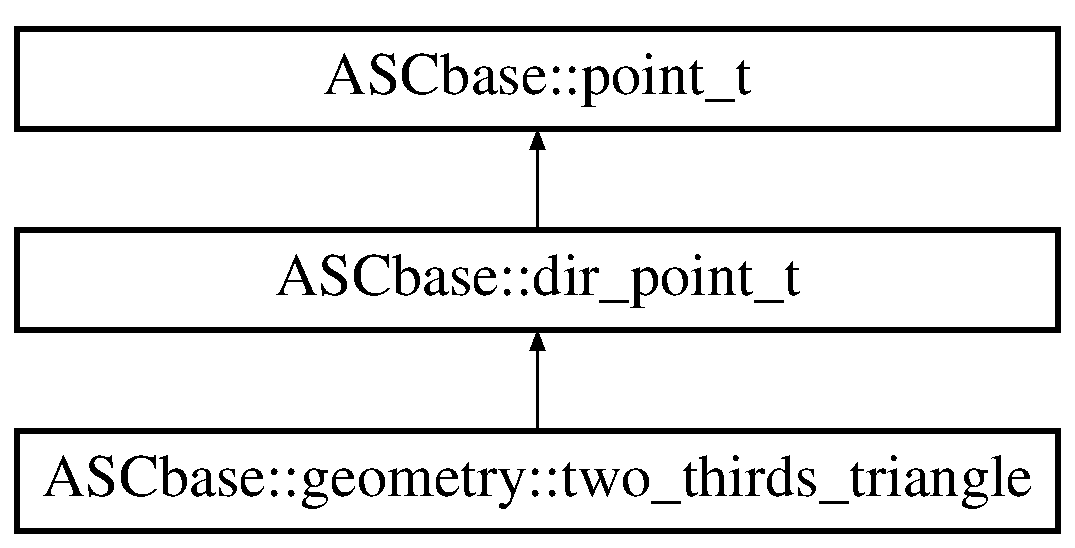
\includegraphics[height=3cm]{classSimSite3D_1_1geometry_1_1two__thirds__triangle}
\end{center}
\end{figure}
\subsection*{Public Member Functions}
\begin{CompactItemize}
\item 
\textbf{two\_\-thirds\_\-triangle} (alloc\_\-t a=ALLOC\_\-POSITION)\label{classSimSite3D_1_1geometry_1_1two__thirds__triangle_c5b749d578f384ebb2f2ebf06b136dad}

\item 
\textbf{two\_\-thirds\_\-triangle} (const \bf{two\_\-thirds\_\-triangle} \&p)\label{classSimSite3D_1_1geometry_1_1two__thirds__triangle_61c17246665ba11761bd28a36450b746}

\item 
const \bf{two\_\-thirds\_\-triangle} \& \textbf{operator=} (const \bf{two\_\-thirds\_\-triangle} \&p)\label{classSimSite3D_1_1geometry_1_1two__thirds__triangle_e4ddddeffcae8e96e30cbe475fc04265}

\end{CompactItemize}
\subsection*{Public Attributes}
\begin{CompactItemize}
\item 
int \bf{triangle\_\-index}\label{classSimSite3D_1_1geometry_1_1two__thirds__triangle_0f34a791ed7ba9f1e116a12da68b1bff}

\begin{CompactList}\small\item\em Index of the triangle in the input file. \item\end{CompactList}\end{CompactItemize}
\subsection*{Private Member Functions}
\begin{CompactItemize}
\item 
void \textbf{do\_\-copy} (const \bf{two\_\-thirds\_\-triangle} \&p)\label{classSimSite3D_1_1geometry_1_1two__thirds__triangle_590f608270791925a9e65210cd3bcc26}

\end{CompactItemize}


\subsection{Detailed Description}
Simple derived class that gives us a unique number for 2/3rds of triangle. 



The documentation for this class was generated from the following file:\begin{CompactItemize}
\item 
Immovable\-Trimesh.H\end{CompactItemize}
